\chapter{Introduction}
The mouse pointer is traditionally controlled using a computer mouse.
The first computer mouse was invented by \emph{Tom Cranston}, \emph{Fred Longstaff} and 
\emph{Kenyon Taylor} as a secret military project in 1952. The project however wasn't 
patented. It would take until 1968 when \emph{Douglas Engelbart} presented the 
first computer mouse to the public. His patent would end in 1987 but at that point the 
computer was already very different from his original. Ever since
it was invented it has been the primary way to control the computer and still is today. Nowadays
there are plenty of solutions out there to challenge the computer mouse.\cite{Mouse40} \cite{Pioneers}

\section{Background}
Since the physical keyboard is rather hard to replace when it comes to typing, this project
will not touch on the matter of constructing any kind of new keyboard. Instead the project
will focus on how to integrate our new approach to controlling the mouse-pointer with the existing
keyboard.\\
In this following section, several already existing solutions are presented to get a grasp
on the good and bad features for controlling the mouse-pointer.\\
Today almost all computer mice are either optical or using some kind of laser. An optical
mouse uses a \emph{light-emitting diode} (LED) and photo-diodes to detect movement on a
surface. Instead of a LED, a laser mouse uses an infrared laser diode to light a surface
beneath the sensor. Their predecessor, the classic mechanical mouse, had a ball that rotated
orthogonal shafts that drove a chopper wheel used to measure the distance moved. The mechanical
mouse had the mainstream market up until 2004 until it was slowly replaced.\\
Not everyone uses desktop computers today. Laptops are becoming more and more popular.
This includes working, gaming and just everyday usage. For example, 55\% of US households
own laptops. That is a 40\% increase from 2010.\\
A laptop usually comes with a trackpad, a touch-sensitive surface below the keyboard
by which the user can control the mouse-pointer on the computer.
The trackpad is a pointing device which has a tactile sensor and is
integrated in the laptop. Since a computer mouse then isn't needed to move
the mouse-pointer, you save a lot of space.\\
Nowadays there's smart-phones and tablets that uses both keyboard, mouse
and display on the same surface. the surface is normally smaller than a computer screen
even on the biggest models.

Since the keyboard is on the screen as well it's hidden away when you don't need it.
The small surface along with the non-physical keyboard can cause problems when doing
trying work on the move. However, the accuracy and comfort of such a surface is un-challanged.\\
Another solution that is often used by dentists takes the form of a pipe formed plastic wheel
at the bottom of the keyboard. This wheel can be moved horizontally to make the mouse-pointer move
left and right, and can be scrolled to make the cursor move up and down. The left and right mouse
buttons are located just below the pipe.

This solution eliminates the need for a regular computer mouse and therefore saves space.\\

\section{Technical background}

\subsection{Infrared light}

\emph{IR-light}, is light composed of wavelengths above the spectrum visible to
the human eye. The human eye can comprehend light in the range of about \emph{380 nm} to about
\emph{700 nm}. IR-light lies in the range of \emph{700+ nm} up to a millimeter.
IR can be used in a variety of areas, like remote temperature sensing, short-range wireless
communications, night-vision and weather forecasting.

\subsection{Arduino}
Arduino is an open-source electronics platform, based on flexible and easy to use hardware.
It is meant for anyone to be able to start developing prototypes of small interactive devices.
The Arduino has got a variety of inputs and outputs where one can easily connect sensors, 
lights, motors and such. Arduinos can be stand-alone projects or communicate with 
software running on a PC or other devices.

\subsubsection{Hardware}
The Arduino used in this project is the Arduino Due. The Due microcontroller board is 
based on the Atmel SAM3X8E Arm Cortex-M3 CPU. Arduino Due is the first Arduino board 
based on a 32-bit ARM microcontroller, and has a large number of digital and analog ports. 
The clock is running at 84 MHz.\cite{ArduinoDue}
\begin{table}
	\caption{Arduino Due hardware.}
	\begin{tabular}{l | r}

		Microcontroller 							&	AT91SAM3X8E \\
		Operating Voltage 							&	3.3V \\
		Input Voltage (recommended)					&	7-12V \\
		Input Voltage (limits)						&	6-20V \\
		Digital I/O Pins 							&	54 (of which 12 provide PWM output) \\
		Analog Input Pins 							&	12 \\
		Analog Output Pins 							&	2 (DAC) \\
		Total DC Output Current on all I/O lines 	&	130mA \\
		DC Current for 3.3V Pin 					&	800mA \\
		DC Current for 5V Pin 						&	800mA \\
		Flash Memory 								&	512KB all available for the user applications\\
		SRAM										&	96 KB (two banks: 64KB and 32KB) \\
		Clock Speed 								&	84 MHz \\

	\end{tabular}
\end{table}

\newpage
\subsubsection{Software}
The microcontroller on the Arduino boards are programmed using the Arduino programming 
language based on Wiring, and using the Arduino development environment based on Processing.
The language is very similar to C/C++ and can therefore be extended using C++ libraries.

There are two basic functions that must be included in every Arduino software, 
the setup() and loop() functions. In setup() the roles of different pins/ports of the Arduino 
are defined, the serial communication with the PC and the Baud rate are defined. In loop() 
the rest of the program is written (except defining new functions).

\subsection{Components}
Since none of the project members has experience in the electronics field, it is 
important to study the basic specifications of the components needed and how they interact 
with each other. 

\subsubsection{Resistors}
A resistor is an essential component in all electronic devices. It is used to add a 
resistance to the circuit independent of current, voltage and external factors like 
temperature and light conditions.

\paragraph{Pull-Up Resistor}
There is always a risk of output anomalies when you connect different circuits and 
components with each other. This will in some cases result in unwanted values while 
measuring the input data.  A pull-up resistor are used to ensure that an input stay 
within the expected measurement levels. This is done by connecting a resistor towards 
its voltage source.

\paragraph{Pull-Down Resistor}
A pull-down resistor work in the same way as a pull-up resistor, but with the 
difference of being  connected towards the ground. This will keep the signal near zero 
volts when no other active component is connected. This will help us control what 
values the photo transistor will output in the state of being in shadow.

\subsubsection{Photo-transistor}
Our Input data is collected with a number of phototransistors. As the name 
suggest, a photo transistor is a photo diode combined with a transistor.  A 
simplification of the transistor would  be to see it as component that regulates 
the amount of current that passes through a particular circuit. The amount of current 
passing through the transistor is controlled with the transistor base, which you operate
with a current. 

This current could come from a photodiode since it will generate a current when, 
but only when, it is exposed to photons of sufficient energy. By changing the current 
flowing through the phototransistor, the sensitivity is calibrated on the photons 
registered. This is a property a conventional photodiode lack.

\begin{figure}[p]
\centering
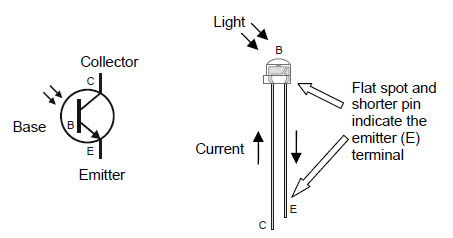
\includegraphics[width=0.8\textwidth]{fig/phototrans}
\caption{Schematic of a phototransistor}
\end{figure}

\subsubsection{Daylight filter}
Another problem is that we need the emitter to match, only, with the phototransistor 
specular characteristics. This is solved by a daylight filter which has a specular 
characteristic that only allow light in the infrared spectrum to pass through. This 
will be placed in front the phototransistor to eliminate all light sources expect our 
own infrared emitters.

\subsubsection{Infrared emitter}
The input data we collect from the phototransistors are generated by a number of infrared 
emitters. A major problem is that each emitter has a fixed angle in which infrared light is 
being emitted. If the angle is too narrow, we would have to compensate with more emitters. 
And if the angle is too wide, we would have inaccurate shadow casting. 
SKRIVA HÄR VILKEN VINKEL VI TOG OCH VARFÖR JUST DEN ÄR SÅ BRA!

\section{Software development}
Since a lot of code will be written by multiple project members during the 
implementation period,  a version control software is needed. We chose to use Bitbucket(GIT).

\section{Related work}
There is a product called \emph{LeapMotion} that uses infrared light and CCD cameras that can
register movements above the device in a 3D space. This enables you to control the cursor with
hand movements. It's small, practical and seems to be very accurate. \emph{LeapMotion} can be
used for other things than just moving the cursor. It can for example be used to rotate animated
objects in a CAD program.\\
\emph{LeapMotion} is set for release the 22th of July 2013.\cite{LeapMotion}

\section{Problems}
One of the first problems that came to mind when developing this prototype is how important 
the design really was. If the design was flawed then the functionality of the prototype would 
suffer severely. Therefore it was very important to think through the design choices.\\

Another problem is how much functionality is decided to be included in the final 
version of the prototype. The more that gets implemented the more work is required
and needs to be planned carefully. However, the basic functions of a computer mouse will be 
included as a minimum.

\section{Goal and purpose}
The purpose of this project is to design and build a prototype that has the basic features of 
a computer mouse. The goal is to replace the computer mouse with a more ergonomic and space-saving
solution. This prototype is mainly meant for making it easier to conduct work in a workenviroment.

\section{Boundaries}
